\section*{Полнота Викиданных}

По данным категории \href{https://ru.wikipedia.org/wiki/%D0%9A%D0%B0%D1%82%D0%B5%D0%B3%D0%BE%D1%80%D0%B8%D1%8F:%D0%9A%D0%BE%D0%BC%D0%BF%D0%B0%D0%BD%D0%B8%D0%B8_%D0%BF%D0%BE_%D0%B0%D0%BB%D1%84%D0%B0%D0%B2%D0%B8%D1%82%D1%83}{Компании по алфавиту} Русской Википедии существует как минимум 10 272 коммерческие организации. Их количество изменяется с каждым днем (обычно, увеличивается) ввиду появления новых организаций, которые заносятся в данный список.

По данным категории \href{https://en.wikipedia.org/wiki/List_of_companies_of_Russia}{List of companies of Russia} Английской Википедии в Росиии существует как минимум 208 коммерческих организаций. Стоит отметить, что в этой категории перечислен рейтинг крупнейших компаний России по объему реализации продукции. Можно сделать вывод, что даже крупные организации не вошли в данный список, не говоря уже про мелкие и средние.

Невозможно получить релевантные данные о количестве коммерческих организаций, так как их количество растёт с каждым днём, а данные о них не хранятся в открытом доступе. Взять, к примеру, ЕГРЮЛ(Единый государственный реестр юридических лиц), который предоставляет данные за плату. \cite{egrul}

"Количество коммерческих организаций, внесенных в госреестр как вновь созданных, в 2014 году составило 420,5 тыс."  свидетельствуют данные на сайте Федеральной налоговой службы (ФНС) России. З0 июня 2015 года вступили в силу приказы Минфина России о том, что данные об имеющихся организациях и информация по ним больше не распространяется в открытом доступе. Данные могут быть предоставлены только органам государственной власти, иным государственным органам, органам местного самоуправления и так далее. Поэтому получить достоверные данные о количестве имеющихся организаций не представляется возможным.

Имеется возможность исследовать полноту с помощью Викиданных. Необходимо вспомнить цифру, полученную вначале, об общем количестве организаций на Викиданных (около 110 000, так как их количество постоянно растет). Обычный пользователь, имеющий общее представление об организациях, возможно, будет заинтересован в том, чтобы посмотреть как выглядит та или иная организация или же в каком месте на карте она расположена.

Чтобы посмотреть, у скольких организаций имеется изображение (то есть, заполнено поле 'image'), необходимо написать следующий скрипт. (Листинг \ref{orgsimages})

\begin{lstlisting}[language=SPARQL,label=orgsimages,caption=Организации с изображением]
#List of organizations with image

SELECT ?org ?orgLabel ?image
WHERE
{
  ?org wdt:P31 wd:Q4830453. #instance of orgs
  ?org wdt:P18 ?image #has image
  
  SERVICE wikibase:label { bd:serviceParam wikibase:language "en"}
}
\end{lstlisting}

\href{https://query.wikidata.org/#%23List%20of%20organisations%20%0A%0ASELECT%20%3Forg%20%3ForgLabel%20%3Fimage%0AWHERE%0A%7B%0A%20%20%3Forg%20wdt%3AP31%20wd%3AQ4830453.%20%23instance%20of%20orgs%0A%20%20%3Forg%20wdt%3AP18%20%3Fimage%0A%20%20%0A%0A%20%20SERVICE%20wikibase%3Alabel%20%7B%20bd%3AserviceParam%20wikibase%3Alanguage%20%22en%22%7D%0A%7D}{SPARQL-запрос}, 2913 записи.

Можно сделать вывод, что количество организаций с изображением равно 2 913. Это не так уж и много, что говорит о неполноте информации.

Построим таблицу из, возможно, популярных свойств в запросах пользователей по организациям (в зависимости от того, кто в чем будет заинтересован насчет организации). Так же, отсортируем ее по убыванию найденных результатов.

\begin{table}[h]
\centering
\begin{tabular}{|l|l|}
\hline
\textbf{Имя свойства} & \textbf{Количество результатов} \\
\hline
inception (Дата создания) & 30995 \\	
\hline
founded by (Кем основана) & 5722 \\
\hline
subsidiary (Дочерние организации) & 3398 \\
\hline
image (Изображение) & 2913 \\
\hline
location (Географические координаты) & 577 \\
\hline
motto (Девиз) & 2 \\
\hline
\end{tabular}
\caption{Запросы на Викиданных}
\label{wdqueries}
\end{table}

Результаты данной таблицы (табл. \ref{wdqueries}) говорят о том, что количество необходимой информации об организациях очень мало, учитывая их общее количество на Викиданных. 

Исследуем российские организации с помощью Викиданных. (Листинг \ref{rusorgs2})

\begin{lstlisting}[language=SPARQL,label=rusorgs2,caption=Организации России]
#List of organizations 

SELECT ?org ?orgLabel
WHERE
{
  ?org wdt:P31 wd:Q4830453. #instance of organizations
  ?org wdt:P17 wd:Q159. #Russia country

  SERVICE wikibase:label { bd:serviceParam wikibase:language "en"}
}
\end{lstlisting}

\href{https://query.wikidata.org/#%23List%20of%20organisations%20%0A%0ASELECT%20%3Forg%20%3ForgLabel%20%3Flocation%0AWHERE%0A%7B%0A%20%20%3Forg%20wdt%3AP31%20wd%3AQ4830453.%20%23instance%20of%20orgs%0A%20%20%3Forg%20wdt%3AP17%20wd%3AQ159.%20%23Russia%20country%0A%0A%20%20SERVICE%20wikibase%3Alabel%20%7B%20bd%3AserviceParam%20wikibase%3Alanguage%20%22en%22%7D%0A%7D}{SPARQL-запрос}, 577 записей.

Запрос вывел 577 организаций. Например, пользователь захотел посмотреть как эти организации расположены на карте. Стоит написать скрипт. (Листинг \ref{rusorgsmap})

\begin{lstlisting}[language=SPARQL,label=rusorgsmap,caption=Карта организаций России]
#Map of organizations 
#defaultView:Map

SELECT ?org ?orgLabel ?location
WHERE
{
  ?org wdt:P31 wd:Q4830453. #instance of orgs
  ?org wdt:P17 wd:Q159. #Russia country
  ?org wdt:P625 ?location #display location

  SERVICE wikibase:label { bd:serviceParam wikibase:language "en"}
}
\end{lstlisting}

\href{https://query.wikidata.org/#%23List%20of%20organisations%20%0A%23defaultView%3AMap%0A%0ASELECT%20%3Forg%20%3ForgLabel%20%3Flocation%0AWHERE%0A%7B%0A%20%20%3Forg%20wdt%3AP31%20wd%3AQ4830453.%20%23instance%20of%20orgs%0A%20%20%3Forg%20wdt%3AP17%20wd%3AQ159.%20%23Russia%20country%0A%20%20%3Forg%20wdt%3AP625%20%3Flocation%0A%0A%20%20SERVICE%20wikibase%3Alabel%20%7B%20bd%3AserviceParam%20wikibase%3Alanguage%20%22en%22%7D%0A%7D}{SPARQL-запрос}, 9 записей.

В результате оказалось очень мало записей с географическими координатами в России. Получить карту организаций не только России, но и всех организаций в мире можно с помощью следующего скрипта. (Листинг \ref{orgsmap})

\begin{lstlisting}[language=SPARQL,label=orgsmap,caption=Карта организаций мира]
#List of organizations 
#defaultView:Map

SELECT ?org ?orgLabel ?location
WHERE
{
  ?org wdt:P31 wd:Q4830453. #instance of orgs
  ?org wdt:P625 ?location

  SERVICE wikibase:label { bd:serviceParam wikibase:language "en"}
}
\end{lstlisting}

\href{https://query.wikidata.org/#%23List%20of%20organisations%20%0A%23defaultView%3AMap%0A%0ASELECT%20%3Forg%20%3ForgLabel%20%3Flocation%0AWHERE%0A%7B%0A%20%20%3Forg%20wdt%3AP31%20wd%3AQ4830453.%20%23instance%20of%20orgs%0A%20%20%3Forg%20wdt%3AP625%20%3Flocation%0A%0A%20%20SERVICE%20wikibase%3Alabel%20%7B%20bd%3AserviceParam%20wikibase%3Alanguage%20%22en%22%7D%0A%7D}{SPARQL-запрос}, 511 записей.

Результат (рис. 3), опять-таки, очень скромный, всего лишь 511 организаций. Количество выведенных организаций с координатами даже меньше, чем общее количество всех организаций в России.

\begin{figure}[h]
	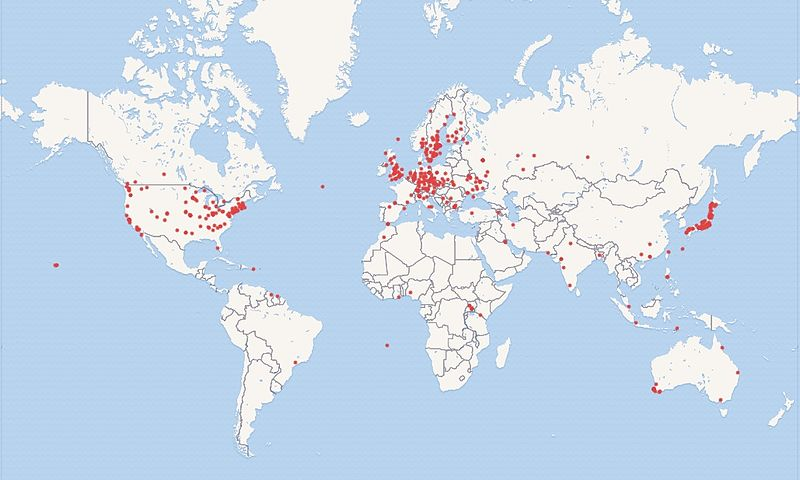
\includegraphics[scale=0.7]{World_organizations_map.jpg}
	\centering
	\caption{Диаграмма дочерних организаций мира}
	\centering
\end{figure}

Проанализировав полученные данные, можно сделать вывод, что данные об организациях на Викиданных заполнены лишь частично. Не имеется достаточной информации, чтобы делать какие-то определенные выводы насчет организаций и их составляющих. Малое количество информации можно было бы объяснить хаотичным появлением и исчезновением организаций (выживать в условиях конкуренции и существующей экономики непросто). Но информация даже о таких крупнейших организациях (Apple, Microsoft, Intel) неполна и нуждается в доработке (например, у организации Intel не указан девиз).